\documentclass[12pt]{article}

%\usepackage{extsizes}
%\usepackage{setspace}
\usepackage[T2A]{fontenc}
\usepackage[utf8]{inputenc}
\usepackage[russian]{babel}
\usepackage{indentfirst}

\usepackage{amsmath}
\usepackage{amssymb}
\usepackage{amsthm}
\usepackage{icomma}
\usepackage{multicol}
\usepackage{multirow}

\usepackage{graphicx}
\usepackage{epstopdf}

%\usepackage{longtable}



\usepackage{pgf,tikz}
\usetikzlibrary{arrows}

\definecolor{xdxdff}{rgb}{0.49019607843137253,0.49019607843137253,1.0}
\definecolor{zzttqq}{rgb}{0.6,0.2,0.0}
\definecolor{qqqqff}{rgb}{0.0,0.0,1.0}
\definecolor{yqqqyq}{rgb}{0.5019607843137255,0.0,0.5019607843137255}

\theoremstyle{plain}
 \newtheorem{theorem}{Теорема}
 
 \theoremstyle{remark}
  \newtheorem*{remark}{Замечание}

\theoremstyle{definition} 
\newtheorem{definition}{Определение}



\begin{document}



\begin{titlepage}

\begin{center}

\textsc{\Large Московский физико-технический институт}\\[0.5cm]
\textsc{\large Кафедра дискретной математики}\\[1cm]

\vfill


{ \LARGE \bfseries Метод Нелдера "--- Мида}
\end{center}

\vfill 

\begin{flushright} 
\begin{minipage}{0.5\textwidth}
\begin{flushright}
\normalsize
Работа студентки 2 курса, гр.~295 Ичаловой Дианы\\
\end{flushright}
\end{minipage}
\end{flushright}


\vfill

\begin{center}
{\large Москва\\
2014 г.}
\end{center}

\end{titlepage}


\section{Введение}

Метод Нелдера"---Мида "--- один из наиболее популярных методов безусловной оптимизации, применяемый в случае когда градиент функции неизвестен или отсутствует. Высокая скорость работы, простота реализации и возможность применения к негладким функциям позволяет использовать его во многих задачах, например, в оптимизации целевой функции в машинном обучении или в максимизации функции правдоподобия в математической статистике. Также некоторой вариацией метода является стандартный алгоритм \texttt{fminsearch} в \texttt{MATLAB}.

\section{Постановка задачи} %описание

Пусть на множестве $\mathbb{R}^n$ определена функция $f: \mathbb{R}^n \to \mathbb{R} $. Задачей минимизации функции называется нахождение следующей величины
\[
f_* = \min_{\mathbb{R}^n}f(x),
\]
а также, если возможно, множества $X_* \subset \mathbb{R}^n$, на котором это значение достигается.

\section{Описание}
Впервые метод Нелдера"---Мида был опубликован в 1965 году в \cite{origin}. Алгоритм является симплекс-методом, т.~е. строит последовательность симплексов, сходящихся к точке минимума.

Перед началом работы выбираются коэффициенты, каждый из которых влияет на одну из фаз метода: $\rho$ "--- коэффициент отражения, $\chi$ "--- коэффициент растяжения, $\gamma$ "--- коэффициент сжатия, $\sigma$ "--- коэффициент уменьшения.

Начальный симплекс выбирается исходя из условий задачи так, чтобы точки симплекса находились не очень далеко от предполагаемой точки минимума.

На каждой итерации алгоритма, кроме тех случаев, для которых выполянется шаг~6, точка с наибольшим значением функции в ней заменяется на новую по следующим правилам.

\begin{enumerate}
\item Упорядочим точки симплекса по возрастанию значения функции в них и обозначим $P_1, P_2, \ldots, P_{n + 1}$. Будем называть точку $P_1$ \emph{наилучшей}, а точку $P_{n + 1}$ \emph{наихудшей}.%, а точку  $P_n$ \emph{второй наихудшей}.

\item Посчитаем центр масс всех точек, кроме наихудшей:
\[
\overline{P} = \frac{\sum_{i = 1}^{n} P_i}{n}
\]

\item \textbf{Отражение.} Определим точку 
\[ P_r = \overline{P} + \rho (\overline{P} - P_{n + 1}),
\] 
полученную отражением точки $P_1$ относительно гиперплоскости $P_1P_2 \ldots P_n$ вдоль прямой $P_{n + 1} \overline{P}$.


\begin{center}
\begin{tikzpicture}[line cap=round,line join=round,>=triangle 45,x=1.0cm,y=1.0cm]
\clip(-2.68,-0.52) rectangle (2.86,3.58);
\fill[color=zzttqq,fill=zzttqq,fill opacity=0.1] (0.0,3.0) -- (0.0,0.0) -- (-2.0,1.5) -- cycle;
\draw [color=zzttqq] (0.0,3.0)-- (0.0,0.0);
\draw [color=zzttqq] (0.0,0.0)-- (-2.0,1.5);
\draw [color=zzttqq] (-2.0,1.5)-- (0.0,3.0);
\draw (-2.0,1.5)-- (0.0,1.5);
\draw (2.0,1.5)-- (0.0,1.5);
\begin{scriptsize}
\draw [fill=qqqqff] (0.0,3.0) circle (1.5pt);
\draw[color=qqqqff] (0.18,3.3400000000000003) node {$P_1$};
\draw [fill=qqqqff] (0.0,0.0) circle (1.5pt);
\draw[color=qqqqff] (0.18,0.33999999999999997) node {$P_2$};
\draw [fill=qqqqff] (-2.0,1.5) circle (1.5pt);
\draw[color=qqqqff] (-1.8199999999999998,1.84) node {$P_3$};
\draw [fill=xdxdff] (0.0,1.5) circle (1.5pt);
\draw[color=qqqqff] (0.18,1.84) node {$\overline{P}$};
\draw [fill=qqqqff] (2.0,1.5) circle (1.5pt);
\draw[color=qqqqff] (2.18,1.84) node {$P_r$};
\end{scriptsize}
\end{tikzpicture}
\end{center}

Если $f(P_1) \le f(P_r) < f(P_n)$, то заменим худшую точку на $P_r$ и завершим итерацию, если $f(P_r) < f(P_1)$, то перейдем к шагу~3, иначе перейдем к шагу~4.

\item \textbf{Растяжение.} Определим точку 
\[ P_e = \overline{P} + \chi (P_r - \overline{P}),
\] 
полученную растяжением отрезка $\overline{P}P_r$ вдоль прямой $P_{n + 1}\overline{P}$ в $\chi$ раз.

\begin{center}
\begin{tikzpicture}[line cap=round,line join=round,>=triangle 45,x=1.0cm,y=1.0301507537688441cm]
\clip(-2.54,0.06) rectangle (4.5,4.04);
\fill[color=zzttqq,fill=zzttqq,fill opacity=0.1] (-0.14,3.46) -- (-0.14,0.46) -- (-2.14,1.96) -- cycle;
\draw [color=zzttqq] (-0.14,3.46)-- (-0.14,0.46);
\draw [color=zzttqq] (-0.14,0.46)-- (-2.14,1.96);
\draw [color=zzttqq] (-2.14,1.96)-- (-0.14,3.46);
\draw (-2.14,1.96)-- (-0.14,1.96);
\draw (1.86,1.96)-- (-0.14,1.96);
\draw (1.86,1.96)-- (3.8600000000000003,1.96);
\begin{scriptsize}
\draw [fill=qqqqff] (-0.14,3.46) circle (1.5pt);
\draw[color=qqqqff] (0.04000000000000001,3.8000000000000003) node {$P_1$};
\draw [fill=qqqqff] (-0.14,0.46) circle (1.5pt);
\draw[color=qqqqff] (0.04000000000000001,0.7999999999999999) node {$P_2$};
\draw [fill=qqqqff] (-2.14,1.96) circle (1.5pt);
\draw[color=qqqqff] (-1.96,2.3000000000000003) node {$P_3$};
\draw [fill=xdxdff] (-0.14,1.96) circle (1.5pt);
\draw[color=qqqqff] (0.04,2.3) node {$\overline{P}$};
\draw [fill=qqqqff] (1.86,1.96) circle (1.5pt);
\draw[color=qqqqff] (2.04,2.3000000000000003) node {$P_r$};
\draw [fill=qqqqff] (3.8600000000000003,1.96) circle (1.5pt);
\draw[color=qqqqff] (4.04,2.3000000000000003) node {$P_e$};
\end{scriptsize}
\end{tikzpicture}
\end{center}

Если $f(P_e) < f(P_r)$, то заменим худшую точку на $P_e$, иначе "--- на $P_r$, и завершим итерацию.

\item \textbf{Сжатие.}
Если $f(P_n) \le f(P_r) < f(P_{n + 1})$ то проведем сжатие наружу, иначе, если $f(P_r) \ge f(P_{n + 1})$, "--- внутрь.
\begin{enumerate} \item \textbf{Сжатие наружу.}
Определим точку 
\[ P_{oc} = \overline{P} + \gamma (P_r - \overline{P}),
\] 
полученную сжатием отрезка $\overline{P}P_r$ вдоль прямой $P_{n + 1}\overline{P}$ в $\gamma$ раз.

\begin{center}
\begin{tikzpicture}[line cap=round,line join=round,>=triangle 45,x=1.0cm,y=1.0148514851485149cm]
\clip(-3.1,0.34) rectangle (3.9,4.38);
\fill[color=zzttqq,fill=zzttqq,fill opacity=0.1] (-0.68,3.76) -- (-0.68,0.76) -- (-2.68,2.26) -- cycle;
\draw [color=zzttqq] (-0.68,3.76)-- (-0.68,0.76);
\draw [color=zzttqq] (-0.68,0.76)-- (-2.68,2.26);
\draw [color=zzttqq] (-2.68,2.26)-- (-0.68,3.76);
\draw (-2.68,2.26)-- (-0.68,2.26);
\draw (1.32,2.26)-- (-0.68,2.26);
\draw (1.32,2.26)-- (3.32,2.26);
\begin{scriptsize}
\draw [fill=qqqqff] (-0.68,3.76) circle (1.5pt);
\draw[color=qqqqff] (-0.5,4.1) node {$P_1$};
\draw [fill=qqqqff] (-0.68,0.76) circle (1.5pt);
\draw[color=qqqqff] (-0.5,1.1) node {$P_2$};
\draw [fill=qqqqff] (-2.68,2.26) circle (1.5pt);
\draw[color=qqqqff] (-2.5,2.6) node {$P_3$};
\draw [fill=xdxdff] (-0.68,2.26) circle (1.5pt);
\draw[color=qqqqff] (-0.5,2.6) node {$\overline{P}$};
\draw [fill=qqqqff] (1.32,2.26) circle (1.5pt);
\draw[color=qqqqff] (1.50,2.6) node {$P_r$};
\draw [fill=qqqqff] (3.32,2.26) circle (1.5pt);
\draw[color=qqqqff] (3.5,2.6) node {$P_e$};
\draw [fill=qqqqff] (0.32,2.26) circle (1.5pt);
\draw[color=qqqqff] (0.54,2.6) node {$P_{oc}$};
\end{scriptsize}
\end{tikzpicture}
\end{center}

Если $f(P_{oc}) \le f(P_r)$, то заменим худшую точку на $P_{oc}$ и завершим итерацию, иначе перейдем к шагу~6.

\item \textbf{Сжатие внутрь.} 
Определим точку 
\[ P_{ic} = \overline{P} - \gamma (P_r - \overline{P}),
\] 
полученную сжатием отрезка $P_{n + 1}\overline{P}$ вдоль прямой $P_{n + 1}\overline{P}$ в $\gamma$ раз.

\begin{center}
\begin{tikzpicture}[line cap=round,line join=round,>=triangle 45,x=1.0cm,y=1.0cm]
\clip(-1.3399999999999999,-0.059999999999998874) rectangle (5.820000000000002,3.9000000000000017);
\fill[color=zzttqq,fill=zzttqq,fill opacity=0.1] (1.14,3.38) -- (1.14,0.38) -- (-0.86,1.88) -- cycle;
\draw [color=zzttqq] (1.14,3.38)-- (1.14,0.38);
\draw [color=zzttqq] (1.14,0.38)-- (-0.86,1.88);
\draw [color=zzttqq] (-0.86,1.88)-- (1.14,3.38);
\draw (-0.86,1.88)-- (1.14,1.88);
\draw (3.14,1.88)-- (1.14,1.88);
\draw (3.14,1.88)-- (5.140000000000001,1.88);
\begin{scriptsize}
\draw [fill=qqqqff] (1.14,3.38) circle (1.5pt);
\draw[color=qqqqff] (1.3200000000000012,3.720000000000002) node {$P_1$};
\draw [fill=qqqqff] (1.14,0.38) circle (1.5pt);
\draw[color=qqqqff] (1.3200000000000012,0.7200000000000013) node {$P_2$};
\draw [fill=qqqqff] (-0.86,1.88) circle (1.5pt);
\draw[color=qqqqff] (-0.6799999999999997,2.2200000000000015) node {$P_3$};
\draw [fill=xdxdff] (1.14,1.88) circle (1.5pt);
\draw[color=qqqqff] (1.32,2.22) node {$\overline{P}$};
\draw [fill=qqqqff] (3.14,1.88) circle (1.5pt);
\draw[color=qqqqff] (3.320000000000002,2.2200000000000015) node {$P_r$};
\draw [fill=qqqqff] (5.140000000000001,1.88) circle (1.5pt);
\draw[color=qqqqff] (5.320000000000001,2.2200000000000015) node {$P_e$};
\draw [fill=qqqqff] (2.14,1.88) circle (1.5pt);
\draw[color=qqqqff] (2.3600000000000017,2.2200000000000015) node {$P_{oc}$};
\draw [fill=qqqqff] (0.14,1.88) circle (1.5pt);
\draw[color=qqqqff] (0.36000000000000065,2.2200000000000015) node {$P_{ic}$};
\end{scriptsize}
\end{tikzpicture}
\end{center}

Если $f(P_{ic}) < f(P_{n + 1})$, то заменим худшую точку на $P_{ic}$ и завершим итерацию, иначе перейдем к шагу~6.

\end{enumerate}
 

\item \textbf{Уменьшение.}

В этом случае определим новые точки
\[
P'_i = P_1 + \sigma (P_i - P_1),\ i = \overline{1, n}.
\]
Эти точки будут вершинами симплекса на следующей итерации.

\begin{center}
\begin{tikzpicture}[line cap=round,line join=round,>=triangle 45,x=1.0cm,y=1.0cm]
\clip(-0.16,-0.07999999999999882) rectangle (6.68,3.899999999999999);
\fill[color=zzttqq,fill=zzttqq,fill opacity=0.1] (2.06,3.36) -- (2.06,0.36) -- (0.06,1.86) -- cycle;
\fill[color=yqqqyq,fill=yqqqyq,fill opacity=0.1] (0.06,1.86) -- (1.06,2.61) -- (1.06,1.11) -- cycle;
\draw [color=zzttqq] (2.06,3.36)-- (2.06,0.36);
\draw [color=zzttqq] (2.06,0.36)-- (0.06,1.86);
\draw [color=zzttqq] (0.06,1.86)-- (2.06,3.36);
\draw (0.06,1.86)-- (2.06,1.8599999999999999);
\draw (4.06,1.86)-- (2.06,1.8599999999999999);
\draw (4.06,1.86)-- (6.06,1.86);
\draw [color=yqqqyq] (0.06,1.86)-- (1.06,2.61);
\draw [color=yqqqyq] (1.06,2.61)-- (1.06,1.11);
\draw [color=yqqqyq] (1.06,1.11)-- (0.06,1.86);
\begin{scriptsize}
\draw [fill=qqqqff] (2.06,3.36) circle (1.5pt);
\draw[color=qqqqff] (2.24,3.6999999999999993) node {$P_1$};
\draw [fill=qqqqff] (2.06,0.36) circle (1.5pt);
\draw[color=qqqqff] (2.24,0.7000000000000007) node {$P_2$};
\draw [fill=qqqqff] (0.06,1.86) circle (1.5pt);
\draw[color=qqqqff] (0.24000000000000002,2.2) node {$P_3$};
\draw [fill=xdxdff] (2.06,1.8599999999999999) circle (1.5pt);
\draw[color=qqqqff] (2.24,2.2) node {$\overline{P}$};
\draw [fill=qqqqff] (4.06,1.86) circle (1.5pt);
\draw[color=qqqqff] (4.239999999999999,2.2) node {$P_r$};
\draw [fill=qqqqff] (6.06,1.86) circle (1.5pt);
\draw[color=qqqqff] (6.24,2.2) node {$P_e$};
\draw [fill=qqqqff] (3.06,1.86) circle (1.5pt);
\draw[color=qqqqff] (3.2800000000000002,2.2) node {$P_{oc}$};
\draw [fill=qqqqff] (1.06,1.86) circle (1.5pt);
\draw[color=qqqqff] (1.2800000000000002,2.2) node {$P_{ic}$};
\draw [fill=qqqqff] (1.06,2.61) circle (1.5pt);
\draw[color=qqqqff] (1.2200000000000002,3.0) node {$P'_1$};
\draw [fill=qqqqff] (1.06,1.11) circle (1.5pt);
\draw[color=qqqqff] (1.2200000000000002,0.7) node {$P'_2$};
\end{scriptsize}
\end{tikzpicture}
\end{center}

\end{enumerate}


\section{Выбор коэффициентов}
Из алгоритма следует, что коэффициенты должны удовлетворять следующим условиям:
\[
\rho > 0,\ \ \chi > 1,\ \ \chi > \rho, \ \ 0 < \gamma < 1,\ \ 0 < \sigma < 1.
\]

Стандартным выбором является следующий набор коэффициентов:
\[ 
\rho = 1,\  \ \chi = 2,\ \ \gamma = \frac12,\ \ \sigma = \frac12.
\]

Однако при больших размерностях данные коэффициенты неэффективны. В \cite{highdimensions} описан выбор коэффициентов в зависимости от размерности задачи:
\[
\rho = 1,\ \ \chi = 1 + \frac2n,\ \ \gamma = \frac34 - \frac{1}{2n},\ \ \sigma = 1 - \frac1n.
\]

\section{Условие завершения}

В качестве условия остановки было выбрано следующее условие:
\[
\sqrt{\frac{\sum_{i = 1}^{n + 1} \left(f(P_i) - f(\overline{P})\right) ^ 2}{n + 1}} < \varepsilon.
\]
По умолчанию $\varepsilon = 10^{-6}$. 


\section{Сходимость}
Несмотря на большую популярность метода, о его сходимости известно очень мало. На данным момент доказана одномерная сходимость при некоторых специальных условиях, а также известно, что при этих же условиях в $\mathbb{R}^2$ метод может расходиться.


\subsection{Некоторые определения}

\begin{definition}
Функция $f$ называется \emph{строго выпуклой}, если для любых $x_1 \ne x_2$ из области определения функции и для любого числа $t \in \left( 0, 1 \right)$ выполнено
\[
f(tx_1 + (1 - t)x_2) < tf(x_1) + (1 - t)f(x_2).
\]
\end{definition}

\begin{definition}
Пусть определена функция $f: D \to \mathbb{R} $, $D \subset \mathbb{R}^n$. Множество 
\[
L_{c}(f) = \{x \in D \mid f(x) \le c \}
\] называется \emph{(нижним) уровневым множеством}.
\end{definition}

\begin{definition}
Будем говорить, что функция $f: D \to \mathbb{R} $, $D \subset \mathbb{R}^n$ \emph{имеет ограниченные уровневые множества}, если для любого $c$ множество $L_{c}(f)$  ограничено.
\end{definition}

\subsection{Сходимость в $\mathbb{R}^1$}

\begin{theorem}[\cite{convergence}]
Пусть $f :  \mathbb{R} \to \mathbb{R}$ "--- строго выпуклая функция с ограниченными уровневыми множествами. Пусть параметры метода удовлетворяют условиям: $\rho > 0,\ \chi > 1,\ \chi > \rho,\ \rho\chi \ge 1, \ 0 < \gamma < 1$. Пусть также начальный симплекс $\Delta_0$ невырожден. \\
Тогда точки симплексов $\{\Delta_k\}$ сходятся к точке глобального минимума.
\end{theorem}

\begin{remark}
Из условия строгой выпуклости и ограниченности уровневых множеств следует, что точка минимума единственна.\\
Условие $\rho\chi \ge 1$ гарантирует, что полученная на шаге растяжения точка $P_e$ лежит вне отрезка (симплекса).
\end{remark}

\begin{theorem}[\cite{convergence}]
Пусть $f :  \mathbb{R} \to \mathbb{R}$ "--- строго выпуклая функция с ограниченными уровневыми множествами. Пусть параметры метода удовлетворяют условиям: $\rho =1 ,\ \chi > 1,\ 0 < \gamma < 1$. Пусть также начальный симплекс $\Delta_0$ невырожден. \\
Тогда существует число $M(\chi, \gamma)$ такое, что метод сходится линейно с шагом $M$ \emph{(M-step linear convergence)}, т.~е.
\[ 
\varlimsup_{k \to \infty} \frac{\left| x_{k + M} - x_{min} \right|}{\left| x_k - x_{min} \right|} = q \in (0, 1).
\]
\end{theorem}

\subsection{Сходимость в $\mathbb{R}^2$}

О двумерной сходимости известно, что с использованием стандартного набора коэффициентов при условии строгой выпуклости функции и ограниченности уровневых множеств,  диаметр симплексов $\{\Delta_k\}$ стремится к нулю. Однако этот факт не гарантирует сходимость. Более того, в \cite{counterexample} приведен общий вид семейства функций, на которых при некотором выборе начального симплекса метод не находит точку минимума. Например,
\[
f(x, y) = \begin{cases} 360  x ^2 + y + y^2, & x \le 0 \\
			     6  x  ^2 + y + y^2, & x > 0 \end{cases}.
\]
Функция $f$ строго выпукла и непрерывно дифференцируема, тем не менее, при $P_1^0 = (0, 0)$, $P_2^0 = (1, 1)$, $P_3^0 = (\frac{1 + \sqrt{33}}{8}, \frac{1 - \sqrt{33}}{8})$ метод сходится в точку $P_1^0$, а не в точку минимума $(0, -\frac12)$, совершая бесконечно много сжатий внутрь.

В 2012 году \cite{convergence2} была доказана сходимость метода без шага растяжения при определенных условиях на функцию $f$.

Открытым остается вопрос, существует ли функция, на которой метод сходится всегда.


\section{Достоинства метода}
\begin{itemize}
\item Не использует градиент функции
\item Высокая скорость сходимости на практике
\item Простота реализации
\item На каждой итерации вычисляется не более 4-х новых значений функции, поэтому метод можно применять, когда вычисление функции является ресурсозатратным

\end{itemize}


\section{Недостатки метода}
\begin{itemize}
\item Находит только локальный экстремум
\item Неэффективен при больших размерностях
\item Неисследованная сходимость
\end{itemize}

\section{Детали реализации}
Для реализации метода был выбран язык \texttt{Python} (версии 3.3) по следующим причинам: 
\begin{itemize}
\item \texttt{Python} ближе к математическому языку, чем другие языки общего назначения
\item \texttt{Python} предоставляет такие же возможности, как языки типа \texttt{MATLAB}, но позволяет просто использовать код в других задачах

\end{itemize}

Для большей точности вычислений использовался модуль \texttt{decimal}.

Все графики в следующей части построены с помощью \texttt{gnuplot}.

\section{Тесты}
Существует много статей, в которых метод протестирован на различных функциях, где главным критерием является количество итераций и ошибка. Поэтому было решено протестировать метод на небольшом количестве функций, сделав упор на исследование зависимости поведения метода от выбора начального симплекса и выявление общих закономерностей работы метода.

Во всех запусках набор коэффициентов стандартный, $\varepsilon = 10^{-6}$.

В таблице используются следующие обозначения: $N_r$ "--- количество отражений, $N_e$ "--- количество растяжений, $N_{oc}$ "--- количество сжатий наружу, $N_{ic}$ "--- количество сжатий внутрь, $N_s$ "--- количество уменьшений,  $N$ "--- общее число итераций. 

\subsection{Сферическая функция}
\vspace{-0.6cm}
\begin{align*}
f(x_1, x_2) &= x_1^2 + x_2^2\\
f_{min} &= 0  \\
x_{min} &= (0, 0)
\end{align*}

 \noindent
\includegraphics[scale=0.6]{sphere1.eps}
\includegraphics[scale=0.6]{sphere2.eps}


\begin{tabular}{|l| c| c| c| c| c| c| c|}
\hline
  Начальный симплекс &N & $N_r$ & $N_e$ & $N_{oc}$ & $N_{ic}$ & $N_s$ & $\left| x - x_{min} \right|$ \\
\hline
 (-2, -2), (2, -2), (0, 2) & 22 & 1 & 0 & 1 & 20& 0 & 0.0014 \\
(-2,5, -1), (-2,5, 1), (-1,5, 0) & 27  &8 & 0 & 1 & 18 & 0 &0.0009 \\
\hline
\end{tabular}

\subsection{Функция Розенброка}
\vspace{-0.6cm}
\begin{align*}
f(x_1, x_2) &= (1 - x_1) ^ 2 + 100(x_2 - x_1^2)^2 \\
f_{min} &= 0 \\
x_{min} &= (1, 1)
\end{align*}

 \noindent
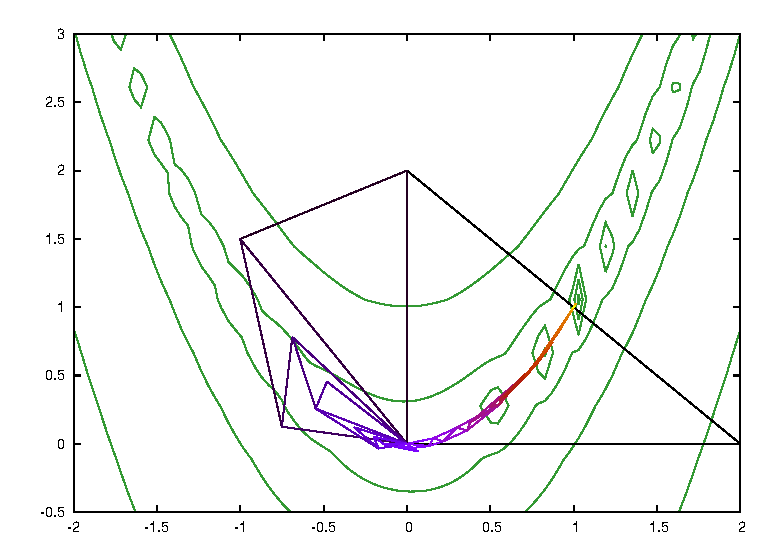
\includegraphics[scale=0.6]{rosenbrock1.eps}
\includegraphics[scale=0.6]{rosenbrock2.eps}
\includegraphics[scale=0.6]{rosenbrock3.eps}
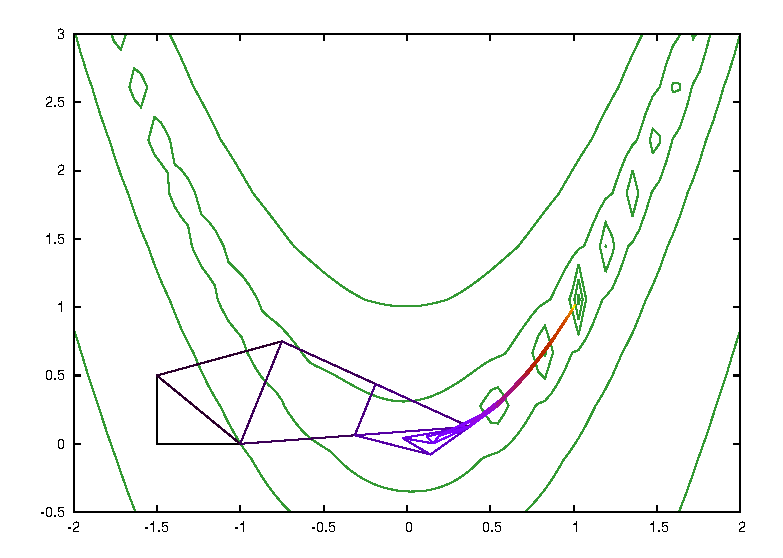
\includegraphics[scale=0.6]{rosenbrock4.eps}

%\begin{table}[h!]
%\begin{center}
\begin{tabular}{|l| c| c| c| c| c| c| c|}
\hline
  Начальный симплекс &N & $N_r$ & $N_e$ & $N_{oc}$ & $N_{ic}$ & $N_s$ & $\left| x - x_{min} \right|$ \\
\hline
 (0, 0), (0, 2), (2, 0) & 49 & 10 & 8 & 6 & 25 & 0 & 0.0035 \\
(0, 0), (0, 2), (-2, 0) & 63  & 29 & 5 & 9 & 20 & 0 & 0.0016 \\
(-0,5, 3), (0,5, 3), (0, 1,5) & 31 & 11 & 0 & 2 & 17 & 1 & 0.0035 \\
(-1.5, 0), (-1.5, 0,5), (-1, 0) & 36 & 4 & 7 & 5 & 19 & 1 & 0.0033 \\
\hline
\end{tabular}
%\end{center}
%\end{table}



\subsection{Функция Химмельблау}
\vspace{-0.6cm}
\begin{align*}
f(x_1, x_2) &= (x_1^2 + x_2 - 11) ^ 2 + (x_1 + x_2^2 - 7) ^ 2 \\
f_{min} &= 0 \\
x^1_{min} &= (3,00, 2,00),\\  x^2_{min} &= (-2,81, 3,13),\\ x^3_{min} &= (-3,78, -3,28),\\ x^4_{min} &= (3,58, -1,85)
\end{align*}

 \noindent
\includegraphics[scale=0.6]{himmelblau1.eps}
\includegraphics[scale=0.6]{himmelblau2.eps}
\includegraphics[scale=0.6]{himmelblau3.eps}
\includegraphics[scale=0.6]{himmelblau4.eps}

\begin{tabular}{|l| c| c| c| c| c| c| c|}
\hline
  Начальный симплекс &N & $N_r$ & $N_e$ & $N_{oc}$ & $N_{ic}$ & $N_s$ & $\left| x - x_{min} \right|$ \\
\hline
 (-2, -1), (-2, 0), (-1, -1) & 30 & 4 & 2 & 6 & 18 & 0 & 0.00035 \\
(-2, 0), (-2, 1), (-1, 0) & 31  &6 &1 & 3 & 21 &  0 & 0.00030 \\
(2, 1), (2, -2), (-2, -0,5) & 34 & 10 & 0 & 1 & 22 & 1 & 0.00036 \\
(-2, -4), (2, -4), (0, 1) & 35 & 10 & 0 & 4 & 20 & 1& 0.00053 \\
\hline
\end{tabular}

\subsection{Функция Экли}
\vspace{-0.6cm}
\begin{align*}
f(x_1, x_2) &= -20 e ^{-0,2 \sqrt{0,5(x_1^2 + x_2^2)}} - e^{0,5(\cos( 2\pi x_1) + \cos(2 \pi x_2))}+ 20 + e\\
f_{min} &= 0  \\
x_{min} &= (0, 0)
\end{align*}

 \noindent
\includegraphics[scale=0.6]{ackley1.eps}
\includegraphics[scale=0.6]{ackley2.eps}
\includegraphics[scale=0.6]{ackley3.eps}
\includegraphics[scale=0.6]{ackley4.eps}


\begin{tabular}{|l| c| c| c| c| c| c| c|}
\hline
  Начальный симплекс &N & $N_r$ & $N_e$ & $N_{oc}$ & $N_{ic}$ & $N_s$ & $\left| x - x_{min} \right|$ \\
\hline
 (-2, -2), (2, -2), (0, 2) & 22 & 1 & 0 & 1 & 20& 0 & 0.0014 \\
(-2,5, -1), (-2,5, 1), (-1,5, 0) & 27  &8 & 0 & 1 & 18 & 0 &0.0009 \\
(-2,5, 0), (-2, 0), (-2, 2) & 27  &4 &2 &3 &18 &0 & 0.0008 \\
(0, 0), (-2.5, 2.5), (2.5, 2.5) & 23  &0 &0 &18 &5 &0 & 0.0000 \\
\hline
\end{tabular}

\vspace{0.8cm}

\subsection{Несколько наблюдений}

Во-первых, видно, что количество уменьшений $N_s$ очень мало, что свидетельствует о том, что почти на каждом шаге происходит уменьшение наихудшего значения в точках симплекса. Во-вторых, отражения позволяют быстро подойти к окрестности точки минимума в случае, если начальный симплекс находится далеко от нее. В-третьих, во всех тестах было очень много сжатий внутрь. Они отвечают за уменьшение диаметра симплекса и стремление к одной точке. В целом, видно, что поведение метода довольно непредсказуемо, что затрудняет его анализ, но обеспечивает хорошую работу на практике.

\nocite{*}

\bibliographystyle{plain}
\bibliography{NelderMead}

\end{document}